\section{What Works, What Fails, and Why}
\label{sec:narrative-results}

\subsection{Physical State Recovery Is Useful but Does Not Locate an Event}

The separate matched-model state study reconstructs 31 unmeasured bus voltages with \BTwoTVE{} mean relative error. Under operating-point shift, regularized AC-feasible recentering closes \EZeroHClosureHalf{}--\EZeroHClosureMax{} of the tested oracle gap. Yet the nuisance information has rank \EZeroHRank{} of \EZeroHDimension{}, and its joint covariance diagnostic remains unreliable. The useful conclusion is target recovery under a stated model, not exact parameter identification or a source-localization guarantee. Full state/mismatch tables and diagnostics remain in the supplement and frozen evidence.

\subsection{Physical Signatures Resolve Stronger Sources, Not Every Weak Pair}

The batch reference evaluates \GlobalHypothesisCount{} hypotheses on \GlobalPhysicalTrajectories{} fresh nonlinear trajectories. Exact-support Top-1 rises from \GlobalWeakTopOne{} for weak pairs to \GlobalFiniteTopOne{} for finite pairs. In the weak regime, even cardinality is imperfect; it nevertheless resolves more often than exact source identity (Fig.~\ref{fig:narrative-resolution}). This is the distinction in \eqref{eq:narrative-separation}: a visible intervention need not have a well-separated location.

The archived retrospective audit associates errors with the closest competing response after amplitude fitting, rather than with a support-only geometric score. The longer-horizon diagnostic increases separation but leaves strongly collinear candidates. Those studies explain a boundary; they do not turn a local numerical condition into a global observability certificate. The original GH31 batch estimator and its denominators remain unchanged.

\subsection{The Causal Gain Is in Load Recognition Under This Contract}

\begin{table}[t]\centering\small
\caption{H04 with the original publication policies. ExtraTrees rows are archived R09 comparators. Load and line columns require the correct family and source emitted before OFF. The 54 realizations repeat 18 interventions across three R/X conditions; they are not 54 independent trials. Normal exposure is only 204 s per method.}
\label{tab:narrative-results}
\setlength{\tabcolsep}{3pt}\begin{tabular}{lrrrr}\toprule
Method & \shortstack{Load\\timely} & \shortstack{Line\\timely} & Extras & \shortstack{Normal\\alarms}\\\midrule
Physical (5 models) & 26/27 & 27/27 & 4 & 0\\
Physical nominal & 27/27 & 27/27 & 7 & 0\\
Archived ET ref. & 0/27 & 27/27 & 3 & 0\\
Archived ET short & 0/27 & 27/27 & 3 & 0\\
Onset witness & 25/27 & 27/27 & 0 & 0\\
\bottomrule\end{tabular}\end{table}


The family breakdown in Table~\ref{tab:narrative-results} is more informative than an aggregate score. In H04, both frozen ExtraTrees adapters and both physical references identify all tested line interventions in time. The physical bank's advantage is concentrated in loads: the five-model version retains \NarMixLoadTimely{}/\NarMixLoadTotal{} timely load decisions and its nominal version \NarNomLoadTimely{}/\NarNomLoadTotal{}, whereas these particular ExtraTrees adapters retain \NarETLoadTimely{}/\NarETLoadTotal{}. This is an observed transfer failure of those frozen adapters on this contract, not proof that supervised learning cannot detect loads. It also cannot be substituted for their historical multi-class hackathon score.

The five-model physical reference detects and eventually attributes \NarMixJoint{}/\NarMixEvents{} realizations, but only \ContMixTimely{} diagnoses arrive before physical OFF. Its nominal reference has \ContNomTimely{} timely diagnoses. Thus detection, eventual attribution and timely attribution give different answers on the same stream. The nominal reference's additional timely decision comes with more extras: \ContNomExtras{} versus \ContMixExtras{}. Model uncertainty has a measured trade-off, not a uniform benefit.

\subsection{Recovery and a New Event Must Remain Competing Explanations}

Figure~\ref{fig:narrative-rolling} exposes the sequence hidden by a count. A load intervention changes several PMU channels, the history bank accumulates evidence, and the active source mass changes. After OFF, the physical state continues evolving. The retained cause/recovery histories allow the observer to explain that trajectory without resetting the network. A later source must compete against both the no-new-event recovery and other interventions.



The out-of-bank BUS31 case shows a remaining timing failure: the source is recovered eventually but too late. The network mixture changes how much mass is assigned to that source, and \eqref{eq:continuous-delta} separates that revision from within-model evidence. This is what the array adds to the explanation. The figure does not establish that a tensor representation alone improves accuracy.

\begin{figure}[!htbp]\centering
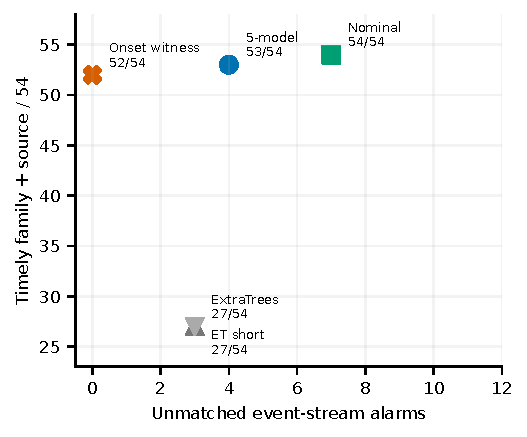
\includegraphics[width=\columnwidth]{figures/generated/narrative_tradeoff.pdf}
\caption{The decision that an accuracy-only table hides. H04 development outcomes trade timely attribution against unmatched event-stream alarms. The onset-witness ablation removes all extras but loses a real BUS16 intervention; it is retained as negative evidence. Labels use 54 paired realizations of 18 interventions and do not imply 54 independent trials.}
\label{fig:narrative-tradeoff}\end{figure}

An additional onset-witness publication ablation reaches zero extras while reducing timely attribution to \ContAdmissionTimely{}/\ContAdmissionTotal{}. It rejects a true BUS16 load with weak early onset evidence. The physical states and underlying masses are inherited, so suppressing the public alarm does not repair the estimator's explanation. We retain this as a negative experiment rather than select it for its zero-extra count. R11 and nominal remain frozen for C01.

\subsection{What Is Still Being Confirmed}

The present development evidence supports causal load/line attribution on a known catalog and shows its failure modes. It does not yet support a final performance claim on C01. The confirmatory executor is running with fixed methods, cases, thresholds and metrics; its completed results will enter the dedicated section below through the same hash-to-table/figure chain. No partial C01 result is used here to choose a variant or revise the method.

\clearpage
\begin{figure*}[p]\centering
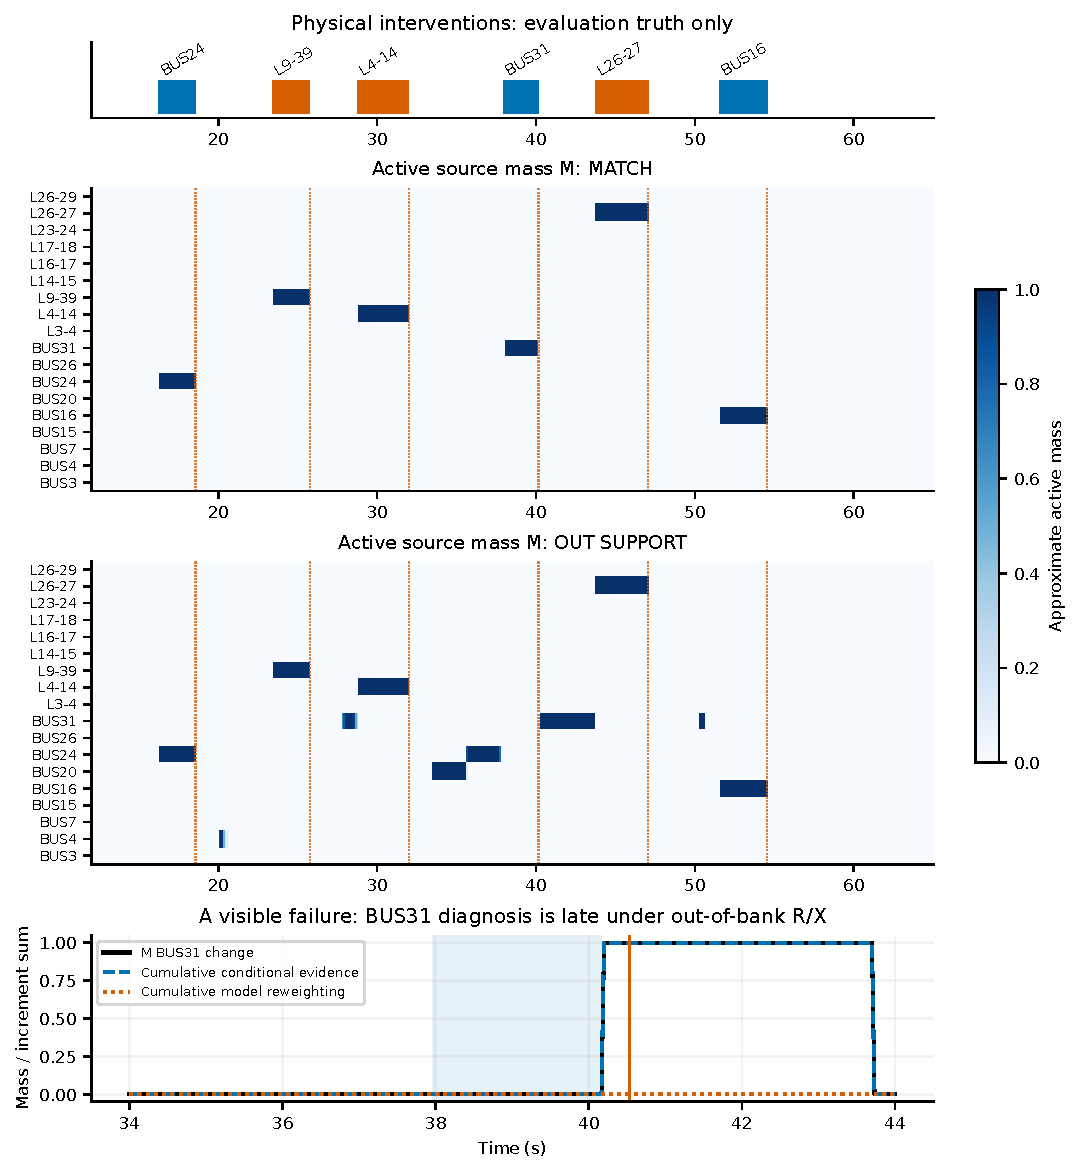
\includegraphics[width=.95\textwidth]{figures/generated/narrative_rolling.pdf}
\caption{From a sequence to an attribution array. Top: reserved physical intervention intervals in fixed H04 parent H002. Middle: causal active masses across the 18 admissible cells for paired nominal and out-of-bank records. Orange dotted lines mark true OFF for evaluation only. Bottom: BUS31 under out-of-bank R/X, with the exact cumulative decomposition of $\Delta M$ relative to 34 s into conditional evidence and model reweighting. The diagnosis marker is later than OFF: an eventual correct source is not a timely success. This is a development illustration, not C01 confirmation or a calibrated probability display.}
\label{fig:narrative-rolling}\end{figure*}
\clearpage
